\problemname{Catfish Farm}

\begin{quote}
\textit{Note:} in this problem, you have to write your solution in C++.
\end{quote}

Bu Dengklek owns a catfish farm. The catfish farm is a pond consisting of a $N \times N$ grid of
cells. Each cell is a square of the same size. The columns of the grid are numbered from $0$ to
$N-1$ from west to east and the rows are numbered from $0$ to $N-1$ from south to north. We
refer to the cell located at column $c$ and row $r$ of the grid ($0 \leq c \leq N-1$,
$0 \leq r \leq N-1$) as cell $(c, r)$.

In the pond, there are $M$ catfish, numbered from $0$ to $M-1$, located at distinct cells. For each
$i$ such that $0 \leq i \leq M-1$, catfish $i$ is located at cell $(X[i], Y[i])$, and weighs $W[i]$
grams.

Bu Dengklek wants to build some piers to catch the catfish. A pier in column $c$ of length $k$ (for
any $0 \leq c \leq N-1$ and $1 \leq k \leq N$) is a rectangle extending from row $0$ to row $k-1$,
covering cells $(c, 0), (c, 1), \ldots, (c, k-1)$. For each column, Bu Dengklek can choose either to
build a pier of some length of her choice or to not build a pier.

Catfish $i$ (for each $i$ such that $0 \leq i \leq M-1$) can be caught if there is a pier directly to
the west or east of it, and there is no pier covering its cell; that is, if
\begin{itemize}
  \item at least one of the cells $(X[i]-1, Y[i])$ or $(X[i]+1, Y[i])$ is covered by a pier, and
  \item there is no pier covering cell $(X[i], Y[i])$.
\end{itemize}

For example, consider a pond of size $N = 5$ with $M = 4$ catfish:
\begin{itemize}
  \item Catfish $0$ is located at cell $(0, 2)$ and weighs $5$ grams.
  \item Catfish $1$ is located at cell $(1, 1)$ and weighs $2$ grams.
  \item Catfish $2$ is located at cell $(4, 4)$ and weighs $1$ gram.
  \item Catfish $3$ is located at cell $(3, 3)$ and weighs $3$ grams.
\end{itemize}

One way Bu Dengklek can build the piers is as follows:

\begin{center}
\begin{tabular}{cc}
  Before the piers are built & After the piers are built \\
  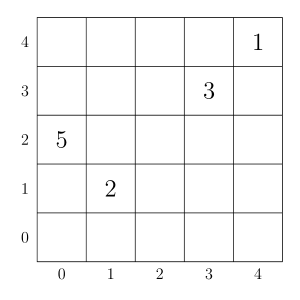
\includegraphics[width=0.35\textwidth]{fish-before.png} &
  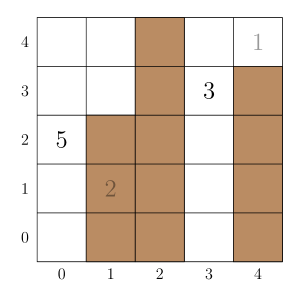
\includegraphics[width=0.35\textwidth]{fish-after.png} \\
\end{tabular}
\end{center}

The number at a cell denotes the weight of the catfish located at the cell. The shaded cells are
covered by piers. In this case, catfish $0$ (at cell $(0, 2)$) and catfish $3$ (at cell $(3, 3)$) can
be caught. Catfish $1$ (at cell $(1, 1)$) cannot be caught, as there is a pier covering its location,
while catfish $2$ (at cell $(4, 4)$) can not be caught as there is no pier directly to the west nor
east of it.

Bu Dengklek would like to build piers so that the total weight of catfish she can catch is as large as
possible. Your task is to find the maximum total weight of catfish that Bu Dengklek can catch after
building piers.

\section*{Implementation Details}
You should implement the following procedure:

\begin{verbatim}
long long max_weights(int N, int M, std::vector<int> X,
                      std::vector<int> Y, std::vector<int> W)
\end{verbatim}

\begin{itemize}
  \item $N$: the size of the pond.
  \item $M$: the number of catfish.
  \item $X$, $Y$: arrays of length $M$ describing catfish locations.
  \item $W$: array of length $M$ describing catfish weights.
  \item This procedure should return an integer representing the maximum total weight of catfish
  that Bu Dengklek can catch after building piers.
\end{itemize}

This procedure is called exactly once.

Your submission must not contain a \texttt{main} function, and must not read from standard input or
write to standard output: a grader is compiled together with your submission and does that for you.
The declaration above lives in \texttt{fish.h}, which is available both to your submission and as an
attachment, so start your file with \texttt{\#include "fish.h"}.

\section*{Constraints}
\begin{itemize}
  \item $2 \leq N \leq 10^5$
  \item $1 \leq M \leq 3 \cdot 10^5$
  \item $0 \leq X[i] \leq N-1$, $0 \leq Y[i] \leq N-1$ (for each $i$ such that
  $0 \leq i \leq M-1$)
  \item $1 \leq W[i] \leq 10^9$ (for each $i$ such that $0 \leq i \leq M-1$)
  \item No two catfish share the same cell. In other words, $X[i] \neq X[j]$ or $Y[i] \neq Y[j]$
  for each $i$ and $j$ such that $0 \leq i < j \leq M-1$.
\end{itemize}

\section*{Scoring}
Your solution will be tested on a set of test groups.
To earn points for a group, you must pass all test cases in that group.

\noindent
\begin{tabular}{| l | l | p{12cm} |}
  \hline
  \textbf{Group} & \textbf{Points} & \textbf{Constraints} \\ \hline
  $1$ & $3$  & $X[i]$ is even for each $i$ \\ \hline
  $2$ & $6$  & $X[i] \leq 1$ for each $i$ \\ \hline
  $3$ & $9$  & $Y[i] = 0$ for each $i$ \\ \hline
  $4$ & $14$ & $N \leq 300$, and $Y[i] \leq 8$ for each $i$ \\ \hline
  $5$ & $21$ & $N \leq 300$ \\ \hline
  $6$ & $17$ & $N \leq 3000$ \\ \hline
  $7$ & $14$ & There are at most $2$ catfish in each column. \\ \hline
  $8$ & $16$ & No additional constraints. \\ \hline
\end{tabular}

\section*{Sample Grader}
A sample grader is available under ``attachments'' at the bottom of this page, together with
\texttt{fish.h} and the sample input. Compile it with your solution and run it on an input file to
try your solution locally. It reads the input in the following format:
\begin{itemize}
  \item line $1$: $N$ $M$
  \item line $2 + i$ ($0 \leq i \leq M-1$): $X[i]$ $Y[i]$ $W[i]$
\end{itemize}
and prints the return value of \texttt{max\_weights} on a single line. That is the format of the
sample data below.

\section*{Explanation of Sample}
The sample is the pond illustrated above. After building the piers as described, Bu Dengklek can
catch catfish $0$ and $3$, whose total weight is $5 + 3 = 8$ grams. As there is no way to build piers
to catch catfish with a total weight of more than $8$ grams, the answer is $8$.
